\chapter{Lecture 6 - Tables}
\begin{definition}[Key and Value]
    A \emph{key} is an independent attribute that can be used as a unique index to look up items in a table, while a \emph{value} is a dependent attribute. \par
    When deciding on the visualization, one should know the number of keys and the number of values in the table, so that different types of tables can be more suitable.
\end{definition}
\section{Scatterplot}
Scatterplot encodes two quantitative attributes (values) using vertical and horizontal spatial position channels, and the mark type is point. It is effective for providing overviews and characterizing distributions, specifically for finding outliers and extreme values. It can also be used to judge the correlation between 2 attributes.\par
\subsubsection{Correlation}
With Visual encoding, the task corresponds to the easy perceptual judgment of noticing whether the points form a line along the diagonal. The stronger the correlation, the closer the points fall along a perfect diagonal line; positive correlation is an upward slope, and negative correlation is a downward slope. In addition, a regression line is often superimposed on the raw scatterplot to show the best fit between attributes. One can even use a transformation to derive a clearer relationship between attributes. It is suited for up to hundreds of points (items) for the scalability issue.

\begin{figure}[htbp]
    \centering
    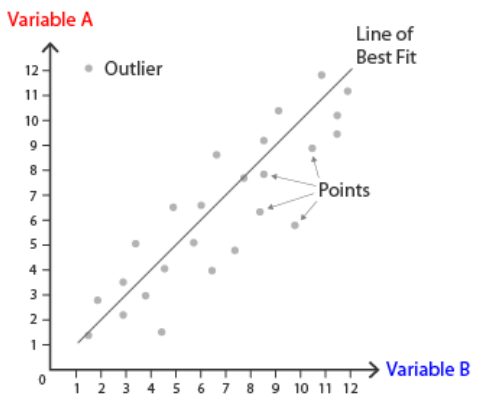
\includegraphics[width=0.35\linewidth]{imgs/lecture6/6.1 scatterplot correlation.png}
    \caption{Scatterplot for feature correlation}
    \label{fig:6.1}
\end{figure}

\subsubsection{Recap: Scatterplot}
\begin{tabularx}{0.8\textwidth} { 
  | >{\raggedright\arraybackslash}l 
  | >{\raggedright\arraybackslash}X | }
    \hline
    Data (What) & Table with 2 quantitative value attributes \\
    \hline
    Encode (How) & Express values with horizontal and vertical spatial position and point marks \\
    \hline
    Task (Why) & Find trends, outliers, distribution, correlation; locate clusters\\
    \hline
    Scale &  hundreds of items\\
    \hline
\end{tabularx}

\section{Bar chart}
A bar chart uses a line mark and usually encodes a categorical or ordinal key attribute using position along the horizontal axis as a channel and a quantitative value attribute with position along the vertical axis. Each bar is in a separate region of space, and there is one for each level of the categorical attribute.\par
It is useful to visualize how a measured quantity is distributed across categories, and also for looking up individual values. Bars are all aligned within a common frame, so that the highest-accuracy aligned-position channel is used.\par
Bars can be ordered alphabetically by the categories, which makes look-up by name easy, but often hinders the meaningful patterns in the dataset. Another ordering is by the values of the quantitative attribute that is encoded by the bar heights; this data-driven ordering makes it easier to see dataset trends. \par
The scalability is a big issue here; to accommodate bars, sufficiently large white space should be allocated so that each bar line mark is distinguishable. \textit{Less is more...}

\subsubsection{Percentage stacked bar chart}
Unlike a simple stacked bar chart, which uses the absolute values. Percentage bar chart uses the normalized values so that the sum of segments in a single bar is 100\%. This can be used to better show the relative difference between quantities in the different groups.

\subsubsection{Recap: Bar charts}
\begin{tabularx}{0.8\textwidth} { 
  | >{\raggedright\arraybackslash}l 
  | >{\raggedright\arraybackslash}X | }
    \hline
    Data (What) & Table with one quantitative value attribute and one categorical key attribute \\
    \hline
    Encode (How) & Line marks, express value attribute with aligned vertical position, separate key attribute with horizontal position \\
    \hline
    Task (Why) & Lookup and compare values\\
    \hline
    Scale &  up to hundreds of levels of key attributes\\
    \hline
\end{tabularx}

\section{Histogram}
A histogram visualizes the distribution of values of a quantitative attribute. It uses the same marks and channels as bar charts, but a histogram usually shows derived or aggregated data; there is no space between bars; it shows the continuous distribution of the data, and thus makes no sense to order bars.

\begin{figure}
    \centering
    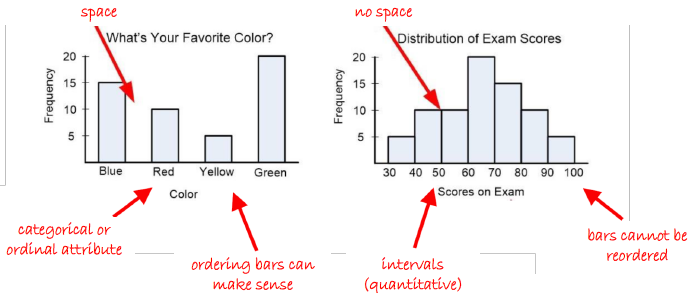
\includegraphics[width=0.5\linewidth]{imgs/lecture6/6.2 bar chart and histogram.png}
    \caption{Difference between a bar chart and a histogram}
    \label{fig:6.2}
\end{figure}

\subsubsection{Recap: Histogram}
\begin{tabularx}{0.8\textwidth} { 
  | >{\raggedright\arraybackslash}l 
  | >{\raggedright\arraybackslash}X | }
    \hline
    Data (What) & Table with one quantitative value attribute \\
    \hline
    Derived (What) & Derived table is the one where one derived ordered key attribute (bin) and one derived quantitative value attribute (item count per bin) \\
    \hline
    Encode (How) & Rectilinear layout, line mark with aligned position to express derived value attribute. Position is judged by key attribute \\
    \hline

\end{tabularx}

\section{Line chart}
A line chart visualizes an ordered key attribute using horizontal position as a channel and a quantitative value attribute using vertical position as a channel. \par
The marks are points and line segments connecting consecutive point pairs. Segments are connection marks to emphasize the ordering of the items along the key ais by explicitly showing the relationship between one item and the next. Thus, they have a stronger implication of trend relationships, making them suitable for the task of spotting trends. Its popular applications include finance, climate studies, public policies ...

\subsubsection{Area Chart} It is a variation of line charts with the area below the line filled in.

\subsubsection{Recap: Line charts}
\begin{tabularx}{0.8\textwidth} { 
  | >{\raggedright\arraybackslash}l 
  | >{\raggedright\arraybackslash}X | }
    \hline
    Data (What) & Table with one quantitative value attribute and one ordered key attribute \\
    \hline
    Encode (How) & Dot chart with connection marks between dots \\
    \hline
    Task (Why) & Show trend\\
    \hline
    Scale &  up to hundreds of levels of key attributes\\
    \hline
\end{tabularx}

\section{Multiple attributes}
\subsection{Bubble Chart}
It is a variation on a scatterplot, accommodated to represent additional attributes, where circle areas and colors can represent additional attributes. One could add even more channels and attributes, but it would also make information decoding much harder. Too many bubbles can make the chart hard to read; therefore, bubble charts have a limited data size capacity. However, this can be solved through interactivity, by, for example, a filter for categories, clicking over a bubble to display hidden information, and so on.

\begin{figure}[htbp]
    \centering
    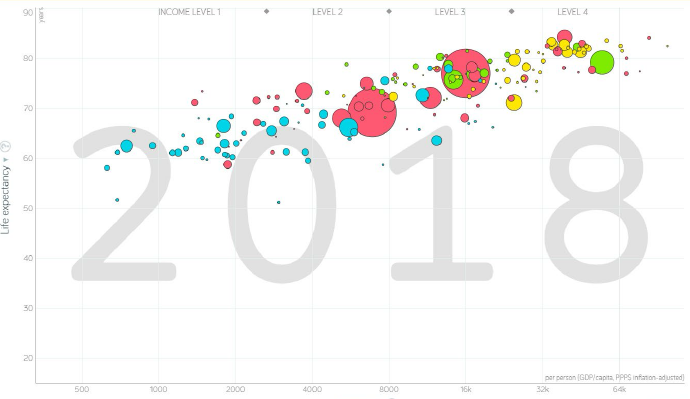
\includegraphics[width=0.3\linewidth]{imgs/lecture6/6.3 bubble chart.png}
    \caption{Bubble chart}
    \label{fig:6.3}
\end{figure}

\subsection{Stacked Bar chart}
It is a more complex glyph for each bar, with multiple sub-bars stacked vertically. It has two key attributes that can have as many composite bars as the number of values for the first key attribute and as many sub-components within each bar as the values for the other key attribute. Both the length of the composite bar and the length of each sub-component encode values, resulting in a multidimensional table.\par
Composite glyphs are arranged horizontally according to the primary key; the secondary key is used to construct the vertical structure of the glyph, and color is often used alongside length coding.

\begin{figure}[htbp]
    \centering
    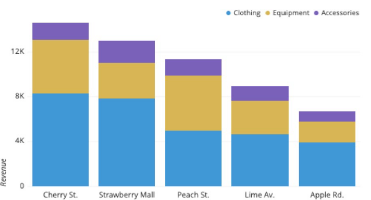
\includegraphics[width=0.4\linewidth]{imgs/lecture6/6.4 stacked bar chart.png}
    \caption{Stacked bar chart}
    \label{fig:6.4}
\end{figure}

In fig~\ref{fig:6.4} shows an example of a stacked bar chart: 
\begin{itemize}[noitemsep]
    \item the full bar height (representing the first key attribute) shows the value for the combination of all items in the stack; 
    \item the height of the full combined bar and the lowest sub-component is easy to read and to compare against each other because they have an aligned starting point
    \item each sub-component is represented with a different color, which represents the second key attribute, it has as many values as the number of sub-components (also color, in this case)
    \item The ordering of stacking is significant, as it determines the patterns that are most easily visible
\end{itemize}

\subsubsection{Recap: Stacked Bar charts}
\begin{tabularx}{0.8\textwidth} { 
  | >{\raggedright\arraybackslash}l 
  | >{\raggedright\arraybackslash}X | }
    \hline
    Data (What) & Multidimensional table with one quantitative value attribute and two categorical key attributes \\
    \hline
    Encode (How) & Bar glyph with length-coded sub-components of value attribute for each category of secondary attribute. Separate bars by category of primary key attribute \\
    \hline
    Task (Why) & Part-to-whole relationship, lookup values, find trends\\
    \hline
    Scale &  up to hundreds of levels for the main axis key attributes. Several levels for the secondary (stacked glyph axis) key attribute\\
    \hline
\end{tabularx}

\subsubsection{Normalized Stacked Bar chart}
It is a variant of stacked bar chart in which the quantitative attribute is normalized, showing proportion instead of absolute values

\subsubsection{Grouped Bar chart}
It is another representation of a stacked bar chart, with two key attributes. The same bar chart is repeated multiple times for the number of categories in the second attribute. It is an excellent tool for the comparison of individual values

\begin{figure}[htbp]
    \centering

    \begin{subfigure}[b]{0.4\linewidth}
        \centering
        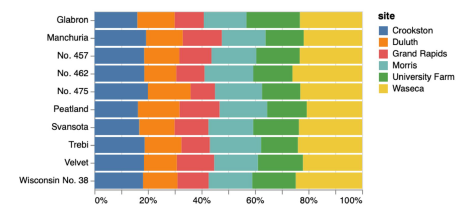
\includegraphics[width=\linewidth]{imgs/lecture6/6.5 normalized stacked bar chart.png}
        \caption{Normalized Stacked Bar chart}
        \label{fig:6.5a}
    \end{subfigure}
    \hfill
    \begin{subfigure}[b]{0.4\linewidth}
        \centering
        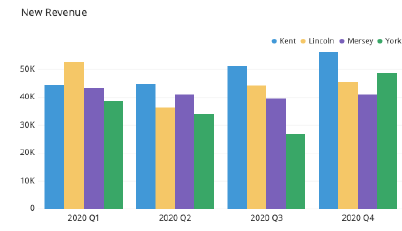
\includegraphics[width=\linewidth]{imgs/lecture6/6.6 grouped bar chart.png}
        \caption{Grouped Bar chart}
        \label{fig:6.5b}
    \end{subfigure}

    \caption{Bar chart variations}
    \label{fig:6.5}
\end{figure}

\subsection{Line chart variations}
\subsubsection{Stacked Line chart}
A variation of a line chart in which values across categories are stacked one on top of each other. It has a big noticeable limitation: it is not good for reading and comparing individual values over time, since the values are stacked, and the shape of lines is affected by the shape of lines below it. This can be somehow mediated through a filter interaction. It can be meaningless for data that shouldn't be summed, like temperature.

\subsubsection{Line chart Series}
It is a collection of lines in the same chart, easy to use, and has high readability, but to be careful to not to overfill the chart with lines.

\subsubsection{Small multiples}
An alternative way to show multiple attributes that hold for all types of charts by creating multiple replicas of the same graph, with each graph in its own chart. It is sometimes more effective than a single plot including too much data.

\subsubsection{Flow maps}
Depict the movement of entities in space and time by placing stroked lines on top of maps. A flow map encode a large amount of multivariate information (thickness, color, etc. can encode additional information)

\begin{figure}[htbp]
    \centering

    \begin{subfigure}[b]{0.32\linewidth}
        \centering
        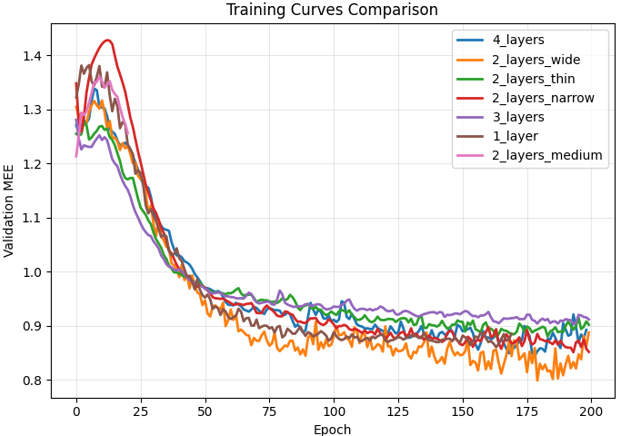
\includegraphics[width=\linewidth]{imgs/lecture6/6.7 line chart series.png}
        \caption{Line chart series}
        \label{fig:6.6a}
    \end{subfigure}
    \hfill
    \begin{subfigure}[b]{0.32\linewidth}
        \centering
        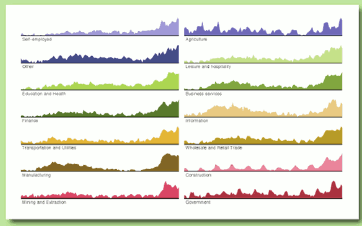
\includegraphics[width=\linewidth]{imgs/lecture6/6.8 small multiples.png}
        \caption{Small multiples}
        \label{fig:6.6b}
    \end{subfigure}
    \hfill
    \begin{subfigure}[b]{0.32\linewidth}
        \centering
        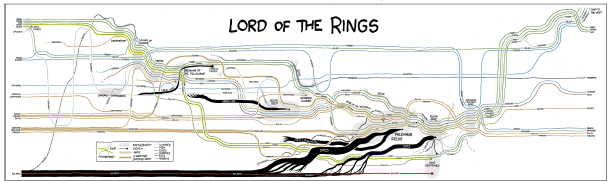
\includegraphics[width=\linewidth]{imgs/lecture6/6.9 flow map.png}
        \caption{Flow map}
        \label{fig:6.6c}
    \end{subfigure}

    \caption{Line chart variations}
    \label{fig:6.6}
\end{figure}

\subsection{Heatmap}
A heatmap is a 2-dimensional matrix alignment to arrange two key attributes and one value attribute. One key is distributed along the rows and the other along the columns; each rectangular cell in the matrix is occupied by an area mark encoding a single quantitative value attribute with color. \par
The use of a heatmap allows us to visually encoding quantitative data with color using small area marks, making it very compact. It is good for overviews with high information density and is highly scalable. Keys can also be ordered to identify patterns, even if it is a categorical attribute (can be ordered according to color). \par
But, its use discriminates a large number of distinct values; only a small number of different levels of the quantitative attribute can be distinguishable, because of the limits of color perception in small, non-contiguous regions.

\begin{figure}[htbp]
    \centering
    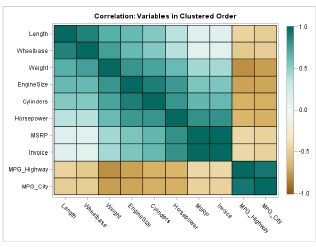
\includegraphics[width=0.5\linewidth]{imgs/lecture6/6.15 heatmap.png}
    \caption{Heatmap}
    \label{fig:6.7}
\end{figure}

\subsubsection{Recap: Heatmap}
\begin{tabularx}{0.8\textwidth} { 
  | >{\raggedright\arraybackslash}l 
  | >{\raggedright\arraybackslash}X | }
    \hline
    Data (What) & Table with one quantitative value attribute and two categorical key attributes \\
    \hline
    Encode (How) & A 2D matrix alignment of area marks, diverging color map \\
    \hline
    Task (Why) & Find clusters, outliers, summarize\\
    \hline
    Scale &  Can have up to one million items; hundreds of levels of categorical attributes; tens of levels of quantitative attributes\\
    \hline
\end{tabularx}

\section{Other visualization tables}
\subsubsection{Wordcloud}
It is a representation of how frequently words appear in a given body of text through the size of the word. It can have various variations in arrangement and color. Mainly used for aesthetic reasons.
\subsubsection{Calligrams}
It is an image created by arranging the texts to form a thematically related image
\subsubsection{Multidimensional icons}
The graph that encode properties of an object in a simple iconic representation. 
\subsubsection{Petals as glyph}
The graph visualize a life index, it maps several variables related to material living conditions and quality of life into petals of different size, to compare well-being across countries. 
\subsubsection{Chernoff faces}
It is introduces based on the assumption that human are good at recognizing faces. Variables are mapped to facial features (width/curvature of mouth, vertical size of face, size/slant/separation of eyes, size of eyebrows...). It needs a legend. \textit{It is not a pre-attentive process...?}

\begin{figure}[htbp]
    \centering
    
    % First row (3 images)
    \begin{subfigure}{0.32\textwidth}
        \centering
        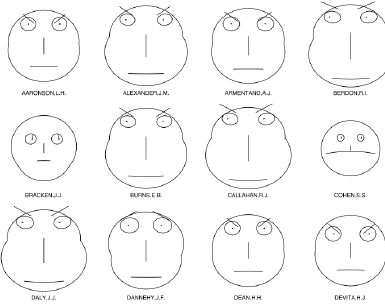
\includegraphics[width=\linewidth]{imgs/lecture6/6.14 chernoff faces.png}
        \caption{Chernoff faces}
        \label{fig:6.8a}
    \end{subfigure}
    \hfill
    \begin{subfigure}{0.3\textwidth}
        \centering
        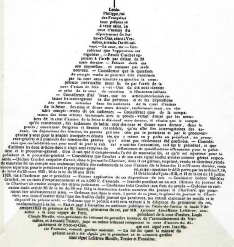
\includegraphics[width=\linewidth]{imgs/lecture6/6.11 calligram.png}
        \caption{Calligram}
        \label{fig:6.8b}
    \end{subfigure}
    \hfill
    \begin{subfigure}{0.3\textwidth}
        \centering
        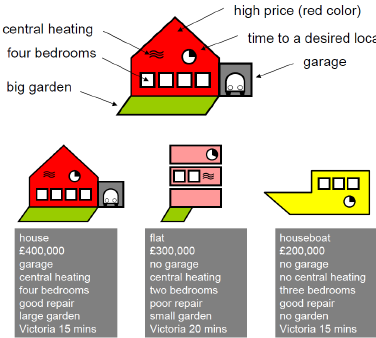
\includegraphics[width=\linewidth]{imgs/lecture6/6.12 multidimentional icons.png}
        \caption{Multidimensional icons}
        \label{fig:6.8c}
    \end{subfigure}

    \vspace{0.5cm}

    % Second row (2 images)
    \begin{subfigure}{0.45\textwidth}
        \centering
        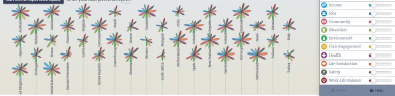
\includegraphics[width=\linewidth]{imgs/lecture6/6.13 petals as glyph.png}
        \caption{Petal as glyph}
        \label{fig:6.8d}
    \end{subfigure}
    \hfill
    \begin{subfigure}{0.45\textwidth}
        \centering
        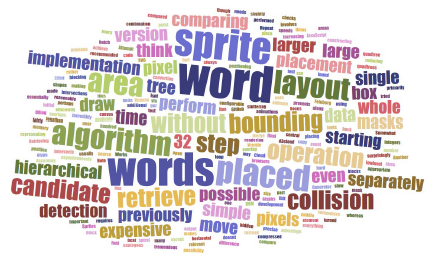
\includegraphics[width=\linewidth]{imgs/lecture6/6.10 wordcloud.png}
        \caption{Wordcloud}
        \label{fig:6.8e}
    \end{subfigure}

    \caption{Other visualization tables}
    \label{fig:6.8}
\end{figure}